\documentclass{article}
\usepackage[utf8]{inputenc}

\usepackage[margin=1in]{geometry}
\usepackage{hyperref}
\usepackage{graphicx}
\usepackage{ulem}

\usepackage{titlesec}

\usepackage{float}
\usepackage{caption}
\usepackage{subcaption}


\setcounter{secnumdepth}{4}
\setcounter{tocdepth}{4}
\titleformat{\paragraph}
{\normalfont\normalsize\bfseries}{\theparagraph}{1em}{}
\titlespacing*{\paragraph}
%{0pt}{3.25ex plus 1ex minus .2ex}{1.5ex plus .2ex}
{0pt}{1.0ex plus 1ex minus .2ex}{0.1ex plus .2ex}

\newcommand{\name}{ECW\ }
\newcommand{\nameNospace}{ECW}
\newcommand{\namep}{ECW.}

\renewcommand{\labelenumii}{\theenumii}
\renewcommand{\theenumii}{\theenumi.\arabic{enumii}}
\renewcommand{\theenumiii}{\theenumii.\arabic{enumiii}}

\usepackage{fancyhdr}
\pagestyle{fancy}

\lhead{ Responsible: Alexander Ekman, Linnea Johnsson, and David Ravanelli \\ Date: \today}  \rhead{Document number: PUSS21419 \\ Version: 1.11}
\renewcommand{\headrulewidth}{0.5pt} 


\title{PFR - Project Final Report}
\author{Team 1}

\begin{document}

\date{}
\maketitle
\thispagestyle{fancy}
\newpage

\section*{Revision History}
\begin{table}[h]
    \centering
    \begin{tabular}{|l|l|p{55mm}|p{35mm}|}
    \hline
    Date & Version & Description & Author \\ 
    \hline\hline 
    2021-10-13 & 1.0 & Section headings and structure & David Ravanelli, Linnea Johnsson, Alexander Ekman  \\
    \hline
    2021-10-13 & 1.1 & First draft and outlines of all sections & David Ravanelli  \\
    \hline
    2021-10-14 & 1.2 & Rough version of all the sections & David Ravanelli \\
    \hline
    2021-10-16 & 1.3 & Completed Phase 1 and 2 sections & David Ravanelli \\
    \hline
    2021-10-18 & 1.4 & Completed Phase 3 section & David Ravanelli \\
    \hline
    2021-10-18 & 1.5 & Draft Section of the Forgotten Issues & Alexander Ekman \\
    \hline
    2021-10-18 & 1.6 & Added section regarding first meeting & Alexander Ekman \\
    \hline
    2021-10-19 & 1.7 & Added section regarding deadlines and rewrote phase 1-2 & Linnea Johnsson \\
    \hline
    2021-10-19 & 1.8 & Completed Phase 4 and summary section & David Ravanelli \\
    \hline
    2021-10-19 & 1.9 & Review Phases 1-4 & Alexander Ekman \& Linnea Johnsson \\
    \hline
    2021-10-19 & 1.10 & Create a "Dos and Don'ts" list & Alexander Ekman \\
    \hline
    2021-10-20 & 1.11 & Proofreading \& rewriting & Alexander Ekman, David Ravanelli \& Linnea Johnsson \\
    \hline
    \end{tabular}
    \label{tab:history}
\end{table}
\newpage

\begin{thebibliography}{widest entry}

    \bibitem{PH} "Programvaruutveckling för Stora System Projekthandledning 2021", Chapter 9, Institutionen för Datavetenskap Lunds Tekniska Högskola, Lunds Universitet, 26 August 2021
    
    \bibitem{SDP} "SDP - Software Development Plan, Team 1 - ETSN05", Team 1, version 1.3
    
    \bibitem{PRD} "PRD - Product Requirements Document, Team 1 - ETSN05", Team 1, version 1.21
    
    \bibitem{STLDD} "STLDD - Software Top Level Design Document, Team 1 - ETSN05", version 1.29
    
   % \bibitem{SDD} "SDD - Software Detailed Design Document, Team 1 - ETSN05"
    
    \bibitem{SVVR} "SVVR - Software Verification and Validation Report, Team 1 - ETSN05", version 1.11
    
    \bibitem{SSD} "SSD - System Specification Document, Team 1 - ETSN05", version 1.6
    
    \bibitem{SPF1} "SPF1 - Software Product Features 1, Team 1 - ETSN05"
    
    \bibitem{SP1} "SP1 - Sprint Planning 1, Team 1 - ETSN05"
    
    \bibitem{SPF2} "SPF2 - Software Product Features 2, Team 1 - ETSN05"
    
    \bibitem{SP2} "SP2 - Sprint Planning 2, Team 1 - ETSN05"
    
    \bibitem{SPF3} "SPF3 - Software Product Features 3, Team 1 - ETSN05"
    
    \bibitem{SP3} "SP3 - Sprint Planning 3, Team 1 - ETSN05"
    
\end{thebibliography}
\newpage

\tableofcontents
\newpage

%information från PH: I samband med projektet ska data samlas in för att bl.a. följa upp nedlagd tid och antal fel. Denna information är en bra grund att ha då man ska starta ett nytt projekt, och dokumenteras därför i en slutrapport. Genom att analysera denna rapport kan man då göra en bra planering både med avseende på tid i allmänhet och resurser som behövs för att rätta de fel som man trots allt gör. I slutrapporten är det således viktigt att man sammanställer insamlad data på ett lämpligt sätt samt att man drar slutsatser utifrån dessa. 
%För alla data som skattades i tidplanen(I SDP!) ska verkligt utfall redovisas. Om tidplanen uppdaterats under projektets gång så ska jämförelse ske med de ursprungliga värdena(Det fick vi ej göra). Eftersom dokumentet skrivs innan sista veckan är färdig så finns inte metricsdata tillgänglig för sista veckan i projektet. Detta kan lösas antingen genom att inte ta med sista veckan i analysen, eller genom att använda skattade värden för sista veckan. 
%Slutrapporten ska omfatta max 20 sidor (exklusive försättsblad, innehålls- förteckning, etc.). Målgruppen för en slutrapport har ofta ont om tid, samtidigt som det är viktigt att rapporten blir läst. Alltså ska omfånget vara begränsat och gäller att välja vad man presenterar och sättet man gör det på.

\section{Introduction}
%what will this report go through?
This report will present an evaluation and overview of the project, its methodology, and its deliverables. The purpose of this is to provide useful information on what went well or bad, why that happened, and how to promote or avoid these situations in future projects. Lastly, the conclusion of this evaluation will be summarized for easy use in future projects.

\section{Phase 1}
\subsection{Historical overview}
%Vad är det som har hänt? Siffror, tabeller och diagram. Jämförelser och uppvisande av data.

Phase 1 was the specification phase where the product requirements, specifications, and project planning was determined and documented in the Product Requirement Document (PRD)\cite{PRD}, and the Software Development Plan (SDP)\cite{SDP}. In this phase the product backlog (SPF1)\cite{SPF1} and the first Sprint Planning (SP1)\cite{SP1} were also produced. 

In the middle of this phase, the whole development team met and discussed possible epics, user stories, and issues for the project. This discussion was seeded by drafts of the PRD \cite{PRD}. This discussion altered some issues in the draft product backlog, and added many new issues which were then put into the official first product backlog SPF1 \cite{SPF1}. During the same meeting the team also decided on which items to bring from the SPF1 into the first sprint, this is documented in the SP1\cite{SP1}. 

The project team was then split into three different internal teams: back end, front end and algorithm. Sprint 1 had not started yet, but the teams were encouraged to meet up and get to know each other. The main purpose for these first internal team meetings was to plan ahead for the upcoming sprint. In the meantime the project owners (POs) set up the project management tools, wrote the drafts for the SDP and the PRD while the scrum master (SM) started to research and prepare for collecting the necessary metrics.

The phase ended with the first formal review where the team got feedback on the written documents that were produced. Most of the feedback was on document details but also a little bit about the team structure. We had failed to document who will be responsible for meetings, taking notes, creating action points and code reviews. This was later clarified.

\subsection{Evaluation \& suggestions of improvements }
%Varför ser det ut som det gör? Analys av de siffror man samlat in. Varför tog det så lång tid i den fasen? Varför blev den modulen så snabbt klar?
%Hur ska man göra för att förbättra de positiva trenderna och få bort de negativa trenderna? Process förbättring mm.

\subsubsection{The joint product backlog and sprint backlog meeting}
Using the PO's draft of the PRD as a springboard for discussing the first product backlog worked very well in getting a useful and effective discussion started. Presenting the PRD draft, creating the product backlog and the first sprint backlog in the very first meeting was very time efficient. However, it would have been beneficial if the PRD was closer to being finished when this meeting took place. This is because the complete use case diagram and list of requirements was a large source of epics and user stories for the product backlog. For this to be implemented, there needs to bee more time for the POs to work on the PRD and get feedback before the first sprint.

\subsubsection{Phase 1 documentation}\label{POBurden}
The main deliverables for phase 1 were the SDP and the PRD. These two documents were large and information heavy, and also the documents which drained the POs the most. Since these documents set the foundation for the project and the POs had the main responsibility for them, they were a heavy burden for the POs. The perceived burden mostly came from the fact that the POs had never seen these kind of documents before, and therefore did not know what they were supposed to look like and, more importantly, contain. 

The guidance that the POs had in this process was mainly the PH book \cite{PH}. The PH book gave some guidance regarding the main topics of each document, but did not go into details on how these topics should be presented. For example, the PRD were to have a technical requirements section but the information in the PH was mainly ascertaining the existence of requirements. Of course the POs could contact Alma for questions, but asking so many questions about the details of all the document sections did not feel like an efficient use of anyone's time. In the light of the available choices, we opted for communication with Alma, other POs, and reading plenty of documents from other companies and courses in order find examples.

Another example, were more but still not enough information was given, was the risk analysis in the SDP. For this section we had practiced formulating risks in the course exercises, but due to time restrictions on these occasions the participants mainly received feedback on what was wrong with their analysis, but not feedback on how it should actually look like. This lead to the POs still feeling unsure how these should be formulated correctly.

The documents were to be produced in phase 1, but the deadline for the first hand in was three days into phase 2. This opened up for a situation were the POs spent a lot of time on phase 1 deliverables during phase 2's first days. This was a necessary evil since other coursework had to be prioritised during the first phase. Especially when taking into account that all the information needed had not been delivered to the POs before the end of the last week of the phase, i.e. the last exercise. This meant that the heavy lifting for the deadline started during the last few days of the phase and continued onto the first days of the next phase. 

Furthermore, the second hand-in for the document was even further into phase 2, meaning the SDP and the PRD were not finished when sprint 1 started. The fact that these documents were not done when the team started working lead to some misunderstandings, and that team members did not refer to them to the extent that they should have. 

In addition to the POs' uncertainty on the documents' contents, and the deadline-to-phase disparity, there was also the fact of they took quite a lot of time to produce. The time estimation on how much time these documents would require was entirely an educational guess on the POs' part. Although, these estimations seemed quite large when they were made it is safe to say they were not enough. Especially for the PRD. To factualize, table \ref{tab:timeDocs} shows the estimated total creation time and revision time per document in comparison to the spent time. It is important to point out that the time spent reporting includes the actual time writing the documents and not necessarily all time spent on discussing and researching the document contents.

\begin{table}[h!]
    \centering
    \begin{tabular}{|c|c|c|c|c|}
    \hline
      Document & Time est. creation & Time spent creation  & Time est. revision & Time spent revision \\
      \hline \hline
      SDP & 24 & 29 & 15 & 12 \\ \hline
      PRD & 24 & 34 & 15 & 19 \\ \hline
    \end{tabular}
    \caption{The SDP's and PRD's time estimation for the project group as well as the time spent by the POs}
    \label{tab:timeDocs}
\end{table}

In order to decrease the POs' work load during the earlier phases, many things can be done. One is to provide example documents of the PRD and SDP so that the POs easier can understand the scope of the documents and how the different information is presented. As discussed earlier, there would have been great benefit to the team having the PRD and SDP finished before the start of sprint 1. This would require the PRD and SDP deadline, and maybe even the second hand-in, to be in the first phase. Since this would create an even heavier workload for the POs, a third PO or a third week to the first phase could be considered.

\subsubsection{Data and team structure}
For this phase we didn't have any data to collect since we did not have access the to time reporting tool yet. Furthermore, no code implementation was done on issues since sprint 1 had not started. The only work done, except for common course work, was early drafts for the PRD and SDP documents and setting up the project management tools. For these deliverables, one can mostly look on the time planned, time spent and the quality of the documents produced. There was a lot of issues finding a free project management tool with the proper features, and in the end a lot of manual work was needed to make GitLab's issue tracker work in a scrum based fashion. This will be discussed further in Section \ref{project_tools}.

Regarding the team structure, feedback showed that the development team appreciated that we split them into sub teams. This made sure that each developer felt useful and could use their skills to full extent. Also, this made the developers feel more confident about the upcoming work. 

From the phase 1 review feedback, we improved the missing details in our documents and also outlined the team's structure and responsibilities more clearly. The scrum master would be responsible for all the meetings, taking notes and creating action points. This seemed like a good setup since the SM was the most intersected role. The architectures got the responsibility to manage the code reviews, since they had the main responsibility, and overview, of the codes structure and future development plans.

\subsubsection{Project management tools}\label{project_tools}
%Förvirringen kring Jira, oneclick, gitlab, epuss osv osv

The project was planned to be managed via Atlassian JIRA, but as the free version only supported 10 developers, our team of 13 had to look for another solution. Multiple other tools were considered, one of them being ClickUp, but since their free version only allowed some objects to be viewed a certain amount of times this option was also scrapped. A locally managed Gitlab server was lastly chosen as both the code repository and the project management tool. This non-premium, and locally managed, service was still lacking some features compared to the premium alternatives. We choose E-puss for time reporting, but due to new legislation, E-puss was discontinued before it was implemented. Time reporting via spreadsheets was implemented in its place, but quite late in the project.

In Gitlab's issue tracker, there were no hierarchical structure for epics, user stories, issues, and sub issues. Instead all entries in the product backlog were added as an issue. Each having a unique ID as X.Y.Z. Where X is the Number of the Epic, Y the number of the user story, and Z the issue number. In this way we were able to organize epics, user stories, and issues in some hierarchical order. However, since Gitlab didn't have the option to sort the list of issues by name, a list in hierarchical order was never achieved.

This method of organizing the issue list was a success considering the tools available, but there were a lot of steps needed for developers to properly add a new issue to the issue tracker:

\begin{itemize}
    \item Create a new issue
    \item Figure out which epic and user story the issue is associated to
    \item Give the issue an appropriate 3 number ID
    \item Add a time estimate
    \item Assign the issue a sprint, priority, and other labels
    \item Move the issue to "Doing"
    \item Do the implementation
    \item Add the time spent
    \item Move the issue to "Done"
\end{itemize}

This lengthy process discouraged developers to add issues, it also wastes a lot of time for the project owners doing the backlog grooming. When the developers add their own issues there could be a lot of incidents where duplicated issues were created, or issues are forgotten. As discussed further in section \ref{forgotten}. This is because it is harder to track the issues manually in such a large unsorted list.

We believe this problem would be solved by using a more advanced project management tool, which is built around the "epics, user story, issues" structure, where manually adding unique identifiers and labels is not a necessity. Furthermore, the exercises in the course were based on JIRA, meaning that all the developers started the course with learning one tool, but then never really had the time to  learn another, less adequate, tool.

This version of Gitlab also did not provide metrics such as burn down charts, so this had to be produced manually by the scrum master. For each sprint the scrum master prepared a spreadsheet which was filled twice a day with the opened and closed issues in order to track the team metrics. This took a lot of time, and opened up for human error. The manual collection of the metrics data and managing the spread sheets filled a majority of the scrum masters time, time which could have been used to help the team. Also, it made it easier for errors to occur.

A premium project management tool would have had time reporting available from the start. If time reporting was available from the start, the team would have been used to tracking their time everyday. This would have increased the chance that they actually could keep track of their spent time for the rest of the project. The other argument for having access to time tracking immediately is that it is hard to remember what you did the first weeks, especially since this phase for most students did not include that much project work. Thus, students probably forgot to retrospectively add these time reports. This results in misleading data on how much time the project members has spent on the course, and for the project group (PG) how much time they spent on getting the project started. This time was significant, especially due to the project management tool ordeal.  

In hindsight, we would have opted for prioritizing a project management tool which had more SCRUM centered functionality. Either by using a paid plan, or setting our group size to 10 in order to use the JIRA software. Even opting for the official Gitlab instead of a locally hosted server could have been beneficial because some functionality such as exporting issue lists and requesting new passwords were not functioning in our version.

\section{Phase 2} %Sprint 1
\subsection{Historical overview}
Phase 2 started off with a stand up meting, the Monday of sprint 1. We started off based on the sprint backlog created with the team in phase 1. We estimated that we would be able to finish 91 story points during the sprint, as shown in figure \ref{fig:Burndown1}. Each issue for the sprint is given an arbitrary weight based on the time the developers thing the issue will need, the value of the weight is the amount of story points for that one issue. The action point from the meeting was that all the sub-teams should meet up and start to plan their assigned issues. During the phase we had stand up meetings on zoom at the beginning and end of each week. During the days in between we had stand up meetings everyday on slack through text. During a meeting between Alma, all the project owners and all the scrum masters decided to use an excel sheet template for time reporting. The Friday of the first week of  sprint 1, phase 2, a formal review was conducted on the deliverables from Phase 1, i.e the PRD, SDP, SPF1, and SP1. During phase 2 the team produced the Software Top Level Design Document (STLDD) \cite{STLDD}, the SPF2 \cite{SPF2}, and the SP2 \cite{SP2}. These documents were to be the topic of discussion during the second formal review coming in phase 3. Phase 2 ended with a sprint retrospective.

\begin{figure}[h!]
    \centering
    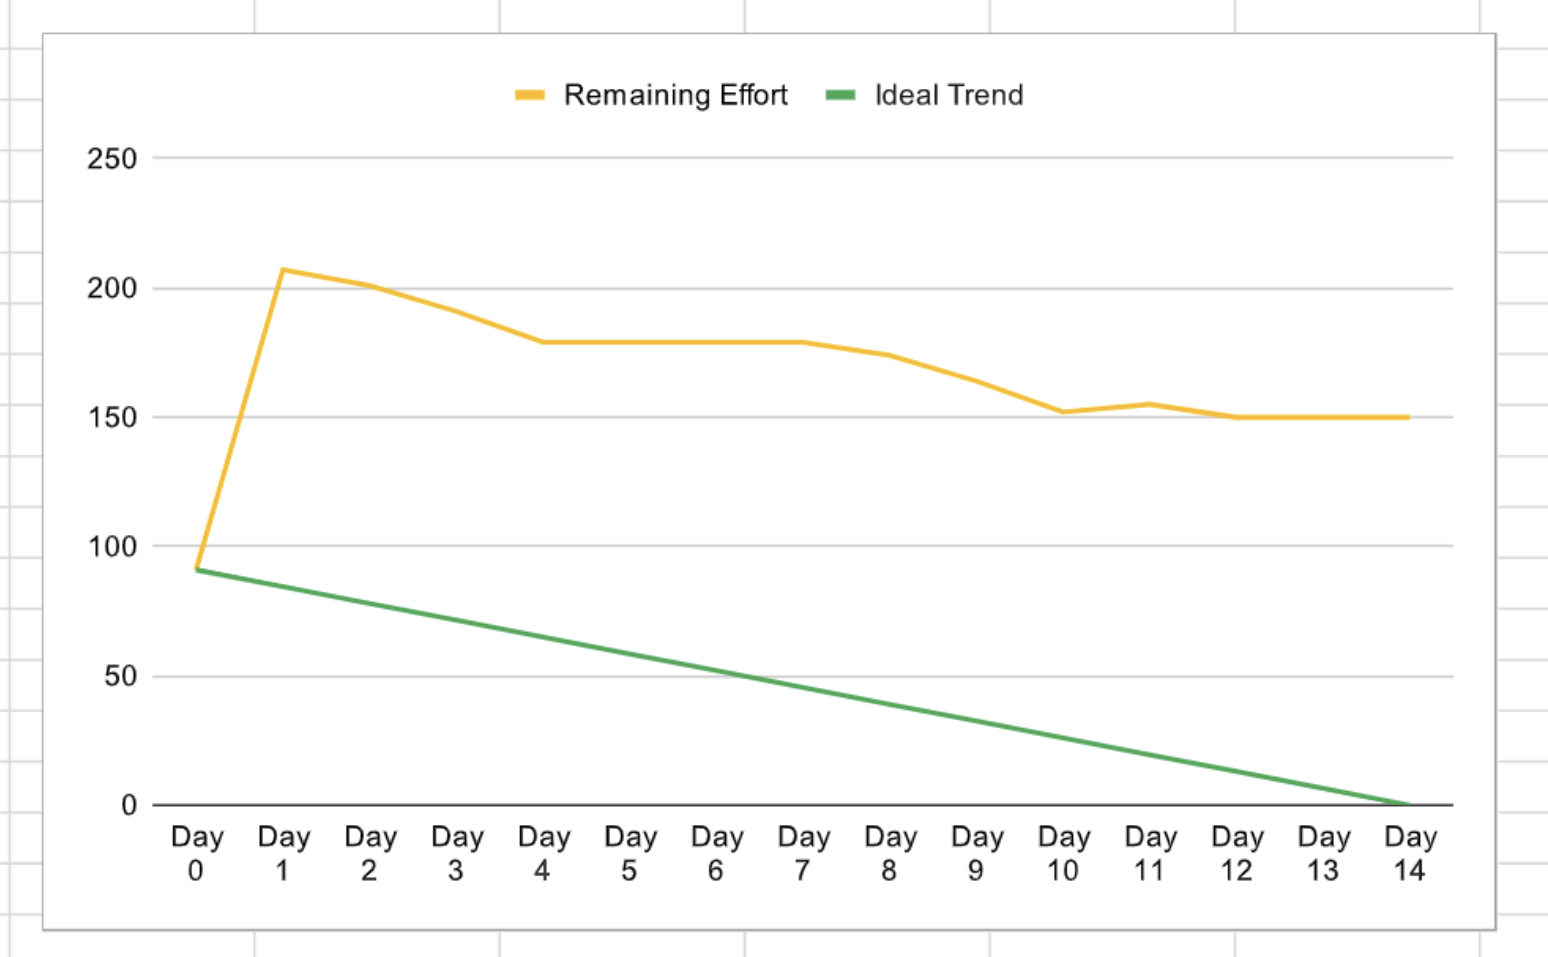
\includegraphics[scale=0.6]{pfrFigures/Sprint1.png}
    \caption{Sprint 1 Burndown chart}
    \label{fig:Burndown1}
\end{figure}

During the sprint retrospective we evaluated the sprint burndown chart as shown in figure \ref{fig:Burndown1}. We recognized that we had underestimated our issues and story points. In the SDP risk analysis section we had already outlined what we need to do if we underestimated sprints. With this information we created action points on how to proceed. The amount of issues needed for the sprint was wrongly estimated but also how many story points that the team would be able to complete.  Out of the estimated 97 story points we only completed 57, i.e. a 62.6 percent completion. During the sprint it is worth noting that we also added a lot of new issues that we had not accounted for in the original SP1, and in some cases not even in the PRD or the SPF1. 

A total of 119 estimated new story points were added. Meaning that we more than doubled our original estimation for the sprint. This happened very early on in the sprint and can be seen in the yellow line that spikes up on day 1 in figure \ref{fig:Burndown1}. During the retrospective meeting we also collected data of team satisfaction as shown in figure \ref{fig:Satisfaction1}. At the phase 2 review (scheduled in the middle of Phase 3) we discussed the STLDD, the SPF2, and the SP2. From the feedback we were told to adjust some small details. These changes were done and the documents were resubmitted, closing the phase 2 chapter.  

\begin{figure}[h!]
    \centering
    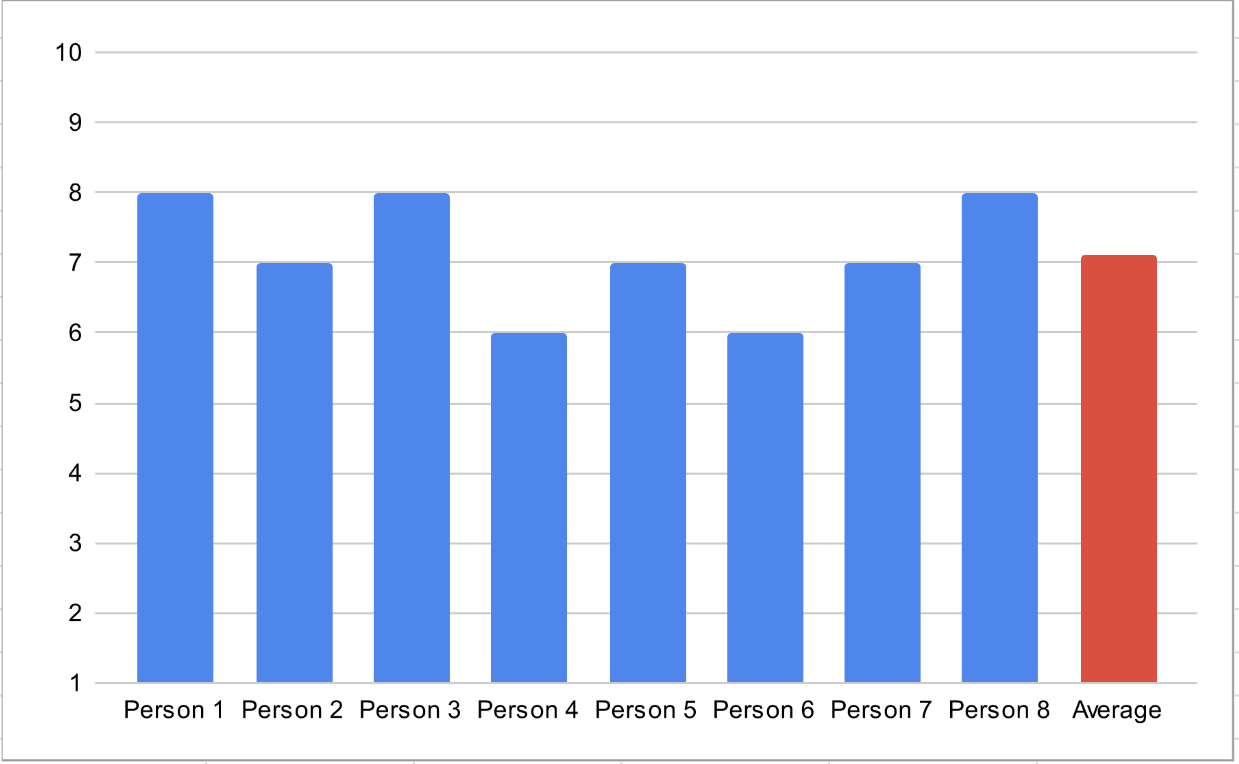
\includegraphics[scale=0.6]{pfrFigures/TeamSatisfaction1.png}
    \caption{Sprint 1 Team Satisfaction chart}
    \label{fig:Satisfaction1}
\end{figure}

\subsection{Evaluation \& suggestions of improvements}
\subsubsection{Data and team structure}

The team satisfaction was on average 7,125 (on a scale of 1-10 were 1 is the lowest and 10 is the highest) as shown in figure \ref{fig:Satisfaction1}. We were happy to already have a high team satisfaction. Our analysis is that the team was happy about the creation of sub-teams, and that they felt comfortable in the current team structure. This led to a decision to continue with the sub-teams, which meant that the team could further develop the structure around sub-teams and that the scrum master helped promote the sub-teams structure. We hoped that this would keep the positive trend and increase the team satisfaction even more for the next sprint. The team satisfaction included the developers and the architects, but not the PG. It would have been interesting, and quite relevant, to have had a separate satisfaction score for the PG.

\subsubsection{Dealing with Large Issues}
As discussed in the sprint retrospective, we had wrongly estimated the amount of issues and story points. Based on the information in the risk analysis in the SDP, we should evaluate and split big issues into smaller issues to make it easier to estimate their story points and the amount of issues. The issues that had not yet been completed were pushed onto the next sprint. Do note that even though there was a large offset between Remaining Effort and Ideal trend in Figure \ref{fig:Burndown1}, the slope of the remaining effort after day 1 is similar to that of the ideal trend. This indicates that the discrepancy has more to do with inexperience creating Epics and user stories, rather than the ability to plan the work and get a certain number of issues done per day.

\subsubsection{Chat standup meetings}
We realised early on during the phase that it was difficult to match everyone's individual schedule for meetings. Every sub-team had their meetings, there were daily stand up meetings, project owner and scrum master meetings and then also meetings with experts. We decided that the sub-team meetings and obligatory course meeting was our priority. This meant that the daily stand up meetings had to be solved in a more flexible way. 

Two zoom meetings each week was possible with our collective schedules, during the other days we had stand up meetings through text on slack. This meant that each developer had between 09:00-12:00 to answer three questions: What did I work on yesterday, what am I going to work on today, and what type of problems has occurred that I need help with. On these stand ups the scrum master informed the team if new information had popped up for the project. The scrum master also reviewed all the questions and decided who needed help and how they should be helped. 

The feedback on the standup meeting setup was positive, so this continued for the duration of the project. The only thing we revised based on the team feedback in this aspect was to let the team have more time to report their availability for the zoom-based standup meetings. Another way to handle this could have been to set two permanent meeting times, but in order to let the team have some flexibility in regard to the schedule we opted for the former way. 

\subsubsection{Weekly Monday meetings}
Another positive take-away from this phase was the weekly Monday lunch meetings with Alma, where scrum masters and project owners from all the groups participated. In one of these we shared our own excel template for the burndown chart and received another template for the time reporting from another group. This shows that these meetings are very valuable and helps all the teams when we share our knowledge together. The template saved our team a lot of work with the time reporting. Although these meetings were valuable, it is worth noting that the time for these meetings were set to 12:30-13:30 without input from the POs and SMs. The mandatory nature of this meeting meant that POs and SMs did not get a Monday lunch break for 7 weeks. This was both stressful and bad for morale. In the future we would suggest using meeting tools like LettuceMeet to plan these meetings.

\section{Phase 3} %sprint 2
\subsection{Historical overview}
Sprint 2 started with a sprint planning meeting. Based on the previous sprint retrospective we decided that we needed to split issues into smaller issues. Each sub-team were also given greater autonomy to choose which issues they wanted to work on. With this information, the backlog, and the sprint log we estimated that we would finish 185 story points this sprint. In this sprint there was no formal review, but the deliverables was the Software Detailed Design Document (SDD) as well as the SPF3 \cite{SPF3} and the SP3 \cite{SP3}. The SDD was the code base and the comments related to it.  

During this sprint we encountered a new problem. The back end team had an issue blocking their upcoming issues. Meaning that they had nothing to work on until the other sub-team resolved the blocking issues. This was caused by a miss-scheduling of the issues. In the SDP's risk analysis we had an action plan on how to handle this. The way to work with damage control for this risk was to allocate more resources and highly prioritise the blocking issue. With this information we had an urgent meeting with the affected sub-teams. At this meeting we got a better understanding of the problem and assigned a developer to resolve the blocking issue. We also decided that the back-end team should help the front-end team with their issues until the blocking issue was resolved. 

During the sprint retrospective we evaluated the sprint burndown chart as shown in figure \ref{fig:Burndown2}. We saw a much greater improvement on how we estimated the sprint. Of the estimated 185 story points we finished 166 story points. This is a 89.7 percent completion of the originally estimated story points. We also added fewer new issues during sprint 2 compared to sprint 1. The newly added issues was this time only 25 extra estimated story points, which can be seen in the yellow line that goes up a little bit during the sprint in figure \ref{fig:Burndown2}. The blocking issue was also discussed. The team thought that our solution where the back-end team helped the front-end team had worked well. The issues was resolved and the back-end team could go back to their original issues. During the meeting we also collected data for the team satisfaction as shown in figure \ref{fig:Satisfaction2}. On a scale of 1-10, we had an average satisfaction of 7.1, which is similar to sprint 1.

\begin{figure}[h!]
    \centering
    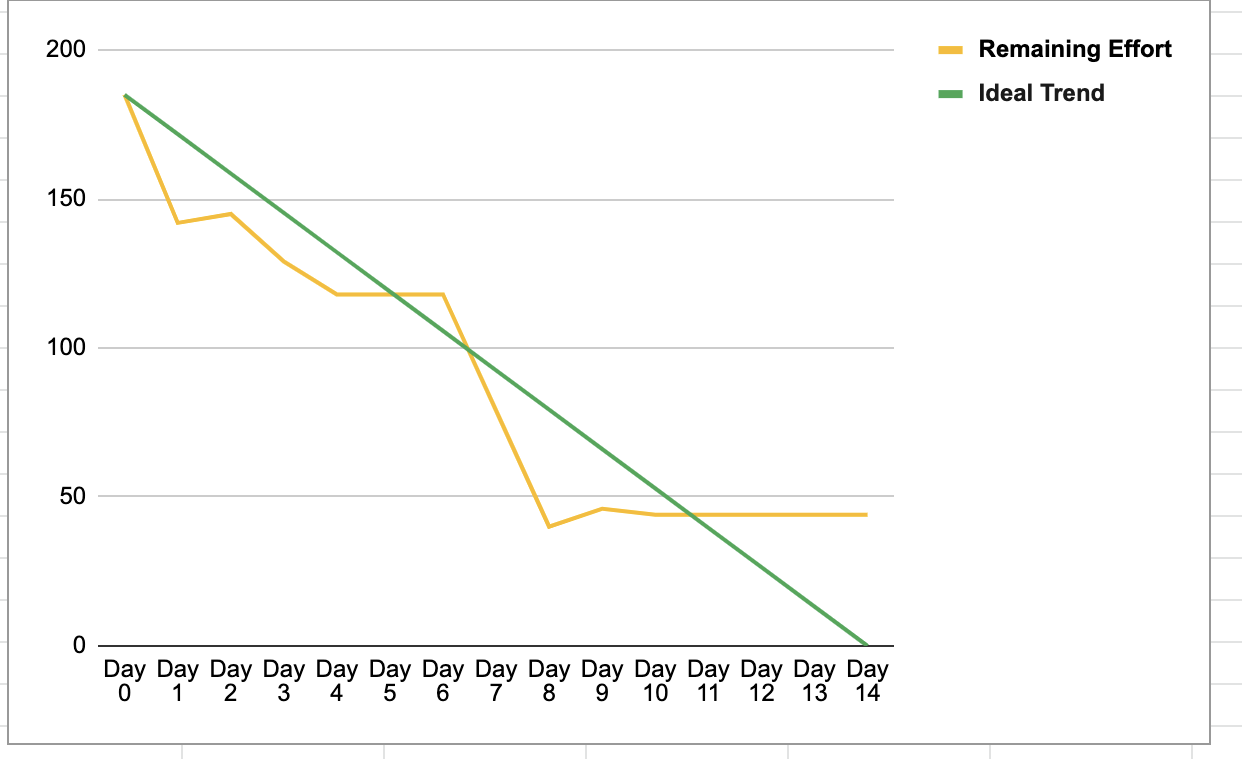
\includegraphics[scale=0.6]{pfrFigures/Sprint2.png}
    \caption{Sprint 2 Burndown chart}
    \label{fig:Burndown2}
\end{figure}

\begin{figure}[h!]
    \centering
    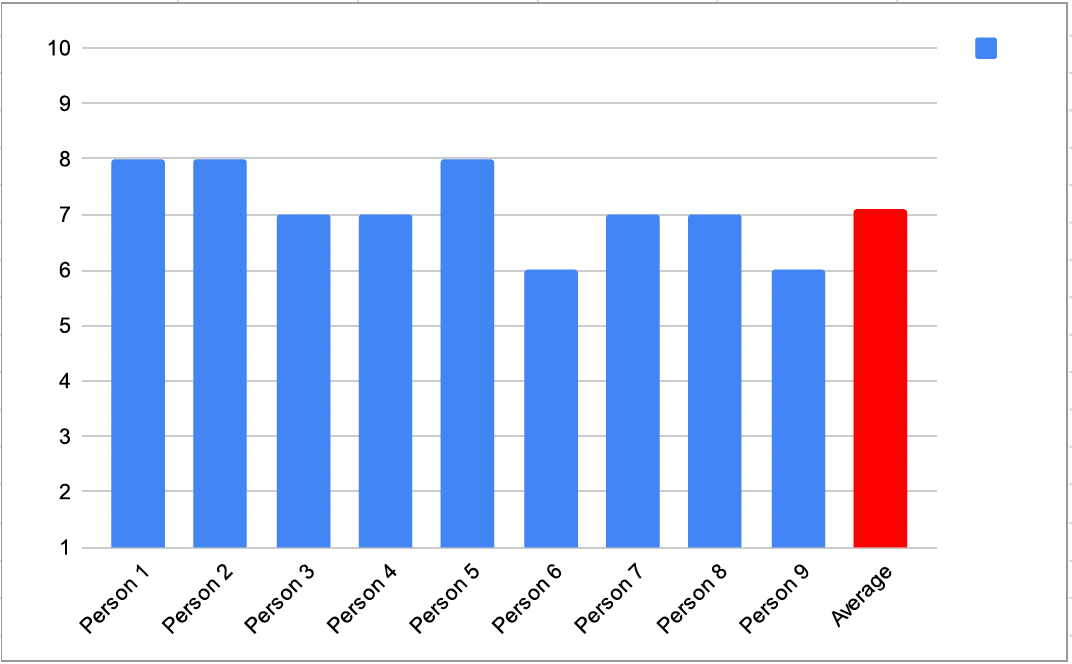
\includegraphics[scale=0.6]{pfrFigures/TeamSatisfaction2.png}
    \caption{Team satisfaction for sprint 2}
    \label{fig:Satisfaction2}
\end{figure}

\subsection{Evaluation \& suggestions of improvements} 


\subsubsection{Data and team structure}
To put it in perspective we had an 89.7 percent completion of the originally estimated story point in sprint 2, compered to the 62.6 percent completion in Sprint 1. Furthermore, when adding the new issues for each sprint this improvement is even more obvious. During sprint one the team completed 26,4 percent of the total story points when taking the new issues into account, while in sprint 2 the team completed 79,0 percent. Another contributing factor to this improvement is that the team now had gotten used to the structure of the project. They have also improved in their work which shows in the data. 

The team satisfaction was roughly the same for Sprint 1 and Sprint 2. This is a good result since it was already high in Sprint 1. It shows that we were doing something right and that the team structure is well received by the developers. The scrum master noticed that in both Sprint 1 and Sprint 2 two people had given a lower score than the rest of the team. We concluded that if we could raise these developers scores we would increase the average of the team satisfaction considerably. Thus, the scrum master contacted the two people that gave a lower score. The SM concluded with them that the main problems that made their satisfaction lower was that there were a lot of blocked merge requests and unclear instructions on what to work on. The two developer took care of this themselves after the discussion with the SM. They presented some suggestions for improvements to the sub-teams, these were included in the next sprint.

\subsection{Employing tactics from the SDP}
The most important improvement of this sprint was our estimation of story points and amount of issues. We realised that when we had written more detailed issues and split them up, it was easier to estimate the amount of story points and also how many issues that were needed from the beginning. This was something that we tried to continue to do and improve even more in Sprint 3. 

During this sprint we had better teamwork within, and between, the sub-teams. With the action points from the SDP and the good teamwork we solved the problem with the blocking issue. The importance of the SDP's risk analysis was made clear when we handled the underestimation of the story points and the blockage problem. Both these situations points to the fact that we had done a great planning before the sprints on how to handle problematic situations. We decided to try to continue this positive trend for the upcoming last sprint by promoting the teams to raise concerns early and to rely on our good planning.

\section{Phase 4} %sprint 3
\subsection{Historical overview}
We started the sprint with a sprint planning meeting. This sprint planning meeting was a little bit different compared to previous sprint plannings. This is because in this sprint we needed to focus on delivering the final product to the customer. This meant that we now had to prioritize issues that would lead to a final product. We decided that each sub-team would meet before the team meeting and decide what type of issues they needed in the sprint to deliver the final product. In addition to the final product, the team were also to produce the Software Verification and Validation Report (SVVR) \cite{SVVR}, the System Specification Document (SSD) \cite{SSD}, and Project Final Report in of itself.

After the sub-team meetings, the product owners and the scrum master met up and prioritized and labeled each issue in Gitlab. The issues were labeled with either "low priority", "medium priority" or "high priority". After this, the whole team met up for the sprint planning. We needed to make sure that for each functionality created by the back-end team, there was also an implementation in the front-end, and vice versa. All these meetings went very well and the sprint could begin.

During the sprint the algorithm team raised some concerns about the match-making algorithm. A meeting with the customer occurred. The algorithm team needed to know what the bare minimum algorithm complexity was acceptable for the customer. The meeting cleared up a lot of questions and the algorithm team could then continue to develop the algorithm. During the sprint retrospective which took place Wednesday of the final week, we saw that we had some problem estimating the amount of issues for this sprint. 

\begin{figure}[h!]
    \centering
    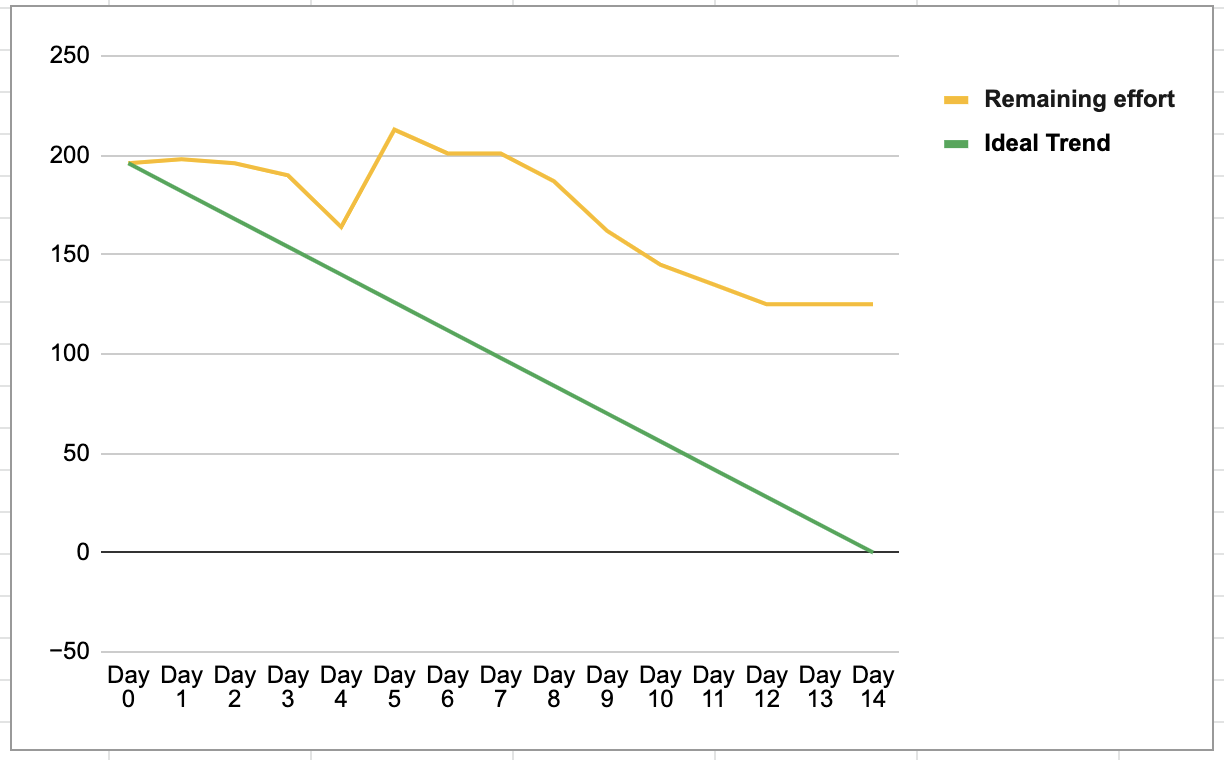
\includegraphics[scale=0.6]{pfrFigures/Sprint3.png}
    \caption{Burn down chart Sprint 3}
    \label{fig:Burndown3}
\end{figure}

During the sprint a lot of new issues popped up as shown in figure \ref{fig:Burndown3}. This meant we had a 62.2 percentage completion of the estimated story points for sprint 3. We had now also collected all the time reporting data for each sprint as shown in figure \ref{fig:timereport} and also the data for the velocity chart as show in figure \ref{fig:Velocity1}. We can see that we now start to estimate roughly the same amount of story points. We landed roughly on 200 estimated story points for a sprint. 

\begin{figure}[H]
    \centering
    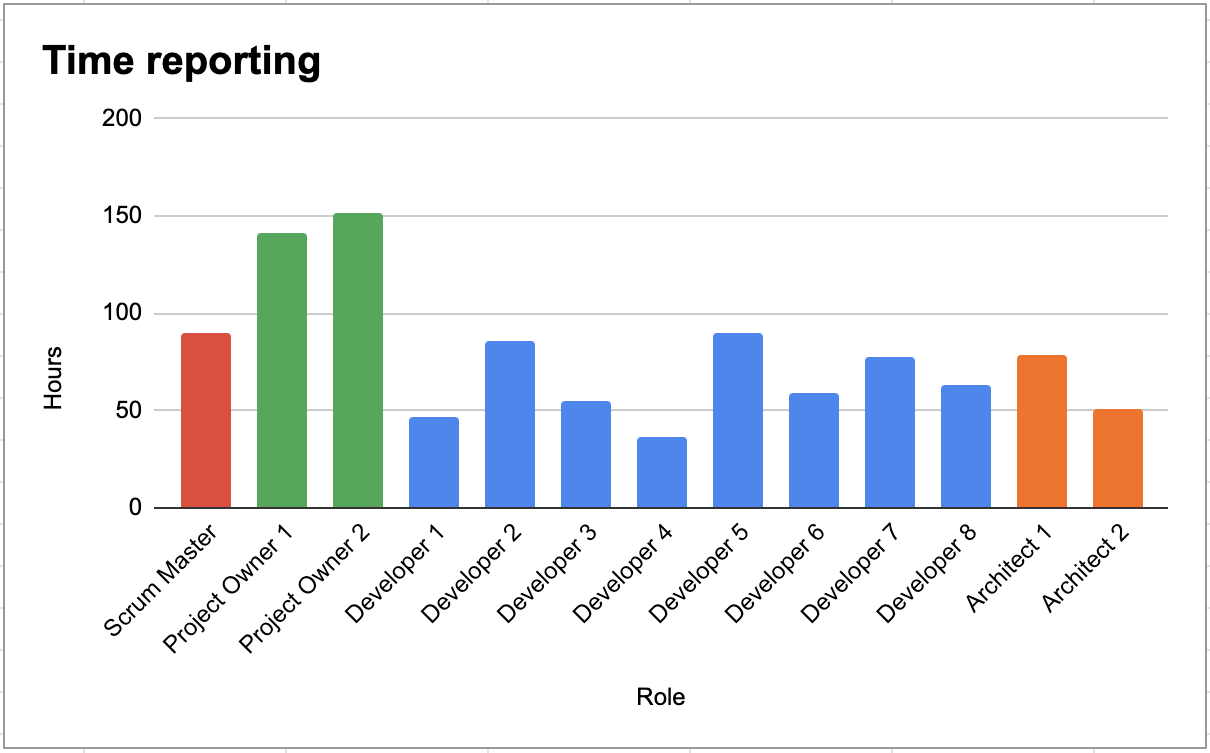
\includegraphics[scale=0.6]{pfrFigures/TimeReporting.png}
    \caption{Time spent on the three sprints combined}
    \label{fig:timereport}
\end{figure}

\begin{figure}[H]
    \centering
    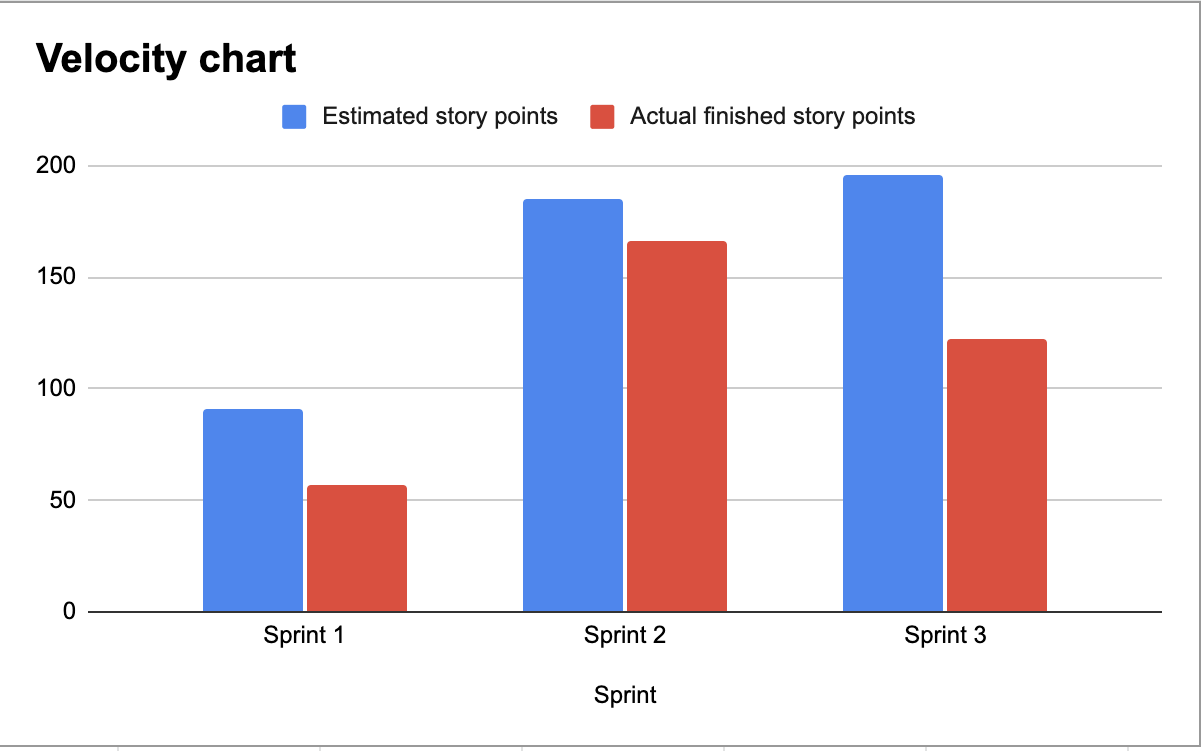
\includegraphics[scale=0.6]{pfrFigures/Velocity.png}
    \caption{Velcotiy chart for all the sprints}
    \label{fig:Velocity1}
\end{figure}

From the time report we discussed that most developers felt they had had a good work load, with not to much or to little work to do. Some mentioned that the last sprint was a bit more hectic than the previous sprints. The architects also felt there had been a fair work load during the project, except for the last sprint were the architectures had more work, working on both code and documentation. This seems natural since they both needed to produce the SVVR and make sure that the project resulted in an acceptable product during this last phase. 

The scrum master also felt that he had enough work during the project. The project owners, on the other hand felt they had too much work during the first, second, and third phase. The overall discussion within the team was positive, we discussed how the team satisfaction improved during the sprint and that the last sprint was very successful which can be seen in both figure \ref{fig:satisfaction3} and figure \ref{fig:totalSatisfaction}. The team satisfaction for sprint 3 rose to 8.1, compared to 7.1 in sprint 2. 

\begin{figure}[H]
    \centering
    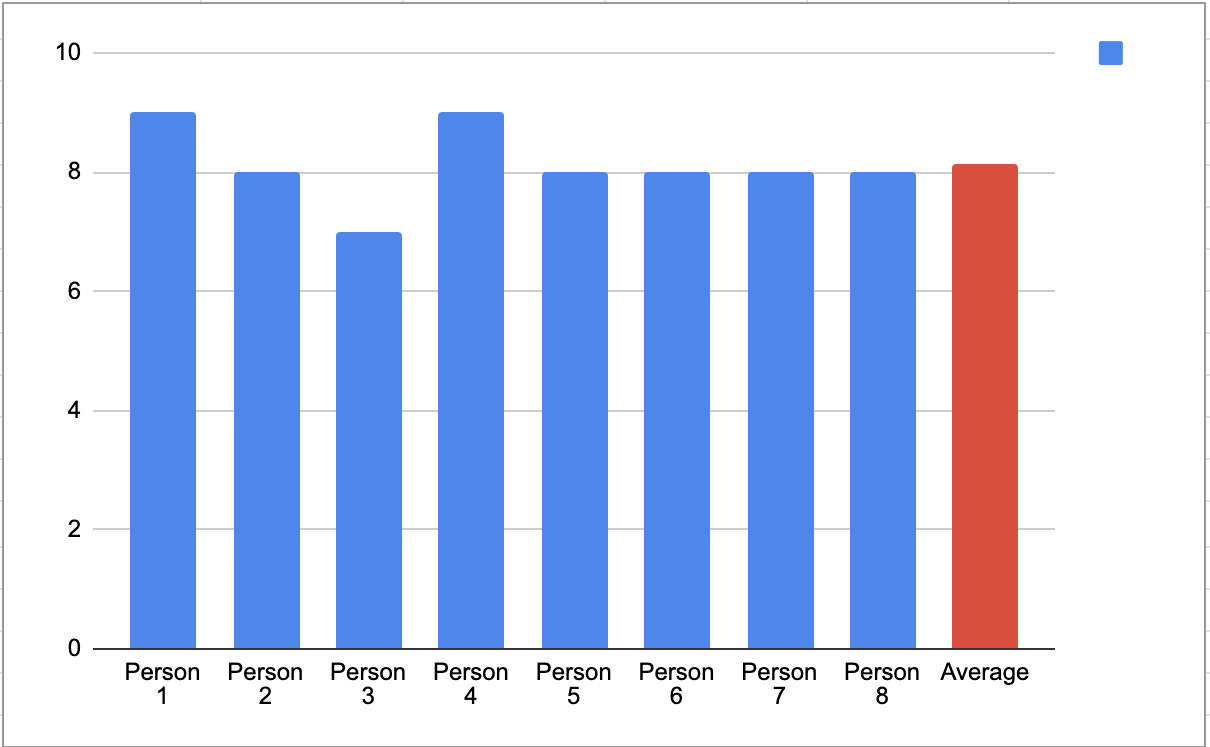
\includegraphics[scale=0.6]{pfrFigures/TeamSatisfactionSprint3.png}
    \caption{Team satisfaction Sprint 3}
    \label{fig:satisfaction3}
\end{figure}

\begin{figure}[H]
    \centering
    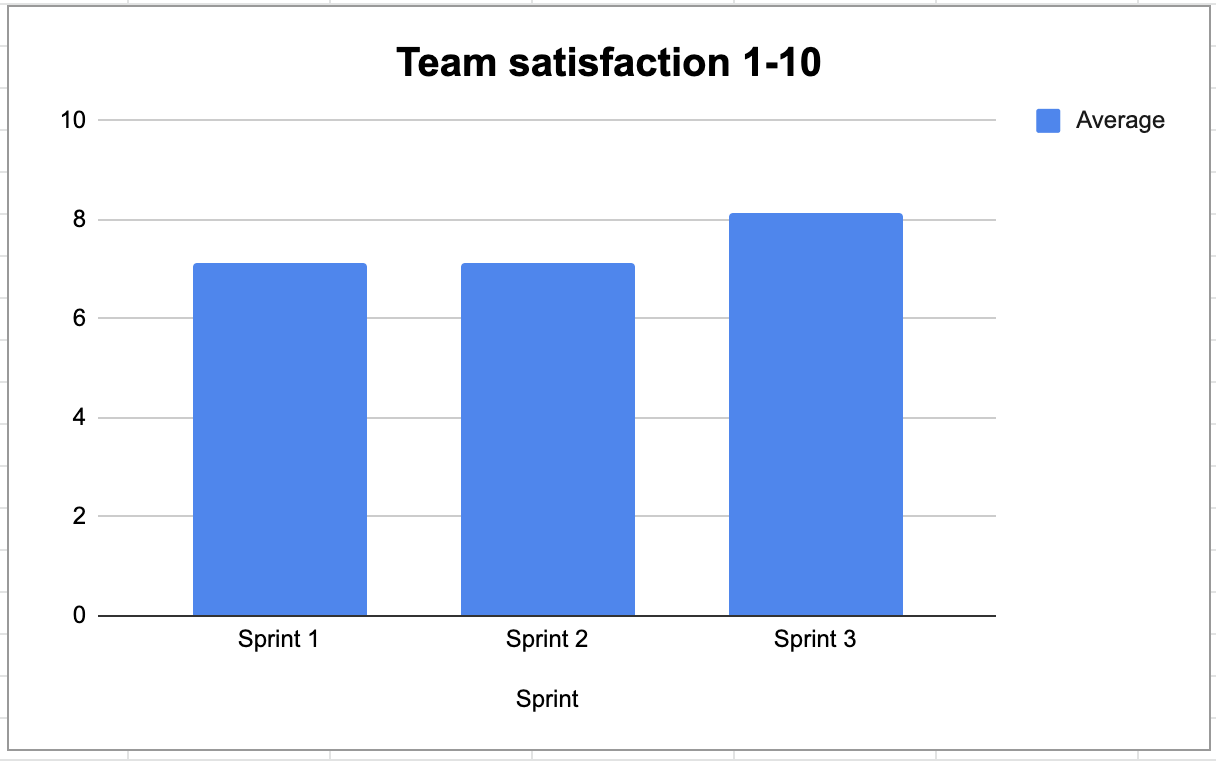
\includegraphics[scale=0.6]{pfrFigures/ToptalSatisfaction.png}
    \caption{Team satisfaction for all sprints}
    \label{fig:totalSatisfaction}
\end{figure}

\subsection{Evaluation \& suggestions of improvements}

\subsubsection{Data \& team structure}
The reason for the new issues being added during the sprint was because of the algorithm implementation. After the meeting with the customer the team got a better idea on what was needed for implementing the algorithm. This meant a lot of new issues appeared. Everything started when we realised that we would not be able to implement an advance algorithm in time. This meant that we needed to know what the bare minimum algorithm complexity was acceptable for the customer. This should preferably had been done before the sprint, so that we could estimate those new issues in the sprint. A better plan and communicating with the customer earlier could have avoided this situation. On the other hand, we realised this at the very beginning of the sprint and raised the concerns early during the phase to the customer. Unfortunately 1-2 days between each meeting makes the time go by fast and before everything was resolved we were 4-5 days into the sprint. The metrics for the burn down chart were affected negatively by this, but in the end a basic version of the algorithm was implemented in time, which met the customer's requirements. Without the new issues this would not have been possible.

%time report
Based on the time report in figure \ref{fig:timereport} it can be concluded that the POs spent the most time on the project during the three sprints. It can also be extracted that the SM and some developers put in quite a lot more time than the rest of the team. This can be the result of many things. One explanation could be that the PG felt more inclined to report their time since they were more aware of its importance. Another explanation could be that since the time reporting was implemented well into the second phase, the habit of this was never formed and the backlogging of the time already spent was less than ideal. Furthermore, some activities might not have been logged even though they should have been, e.g. administrative work or keeping up with slack etc.

To save time for the scrum master the project could have benefited from automatic metric tools. This would have cleared up more time for the SM to help the team, as discussed in section \ref{project_tools}. For the project owners they could have benefited from a third person to share the load, an extra week, or detailed example documents, as discussed in section \ref{POBurden}.

The first sprint deviates from the estimated story points. That is because a lot of the developers were not used to estimating issues. We can see that sprint 2 and sprint 3 are roughly estimated the same amount of story points. This shows that the developers quickly learned how to estimate. As mentioned earlier sprint 3 had a lower completed story points percentage compared to sprint 2. This can be linked to the new issues added for the algorithm. In this sprint the developers had to spend more time on exploring what should be implemented, which took time away from actually implementing issues.

The team satisfaction improved a lot on sprint 3. Previous  sprints had an average team satisfaction of roughly 7.1, this sprint had 8.1. This is a very positive improvement. Thanks to the metrics we could recognize which developers felt less happy. They themselves then solved it very well within their own teams, after the problem was raised by the SM. The developers' analysis was that they by this sprint had a better prioritisation process due to the emerging deadline for the product. They also had a better cooperation between the sub-teams were they had good communication which led to a better distribution of the work load. All of this made the developers feel more happy about the last sprint as shown in the data.

\subsubsection{Continuously updated documentation}
%For the architects sake, there was a mishap in communication that resulted in them spending time on unnecessarily updating the STLDD after its final hand-in. They believed, as did the PG for quite some time, that documentation should be kept up to date even after they were handed in after their formal review. If it had been made clear in the PH that this was not the case, this could have been avoided.
Since the architects were not invited to the weekly PO+SM meetings, this resulted in them spending time updating the STLDD even though it was not expected to be continuously updated. The architects believed, as did the PO+SM for quite some time, that the documentation should be kept up to date after they were handed in. If the PH book would have stated that this was not the case, this could have been avoided.



\subsubsection{The List of Forgotten Issues} \label{forgotten}
In the middle of phase 4 the product owners and scrum master found an interesting sub group of issues in the product backlog. If the issues were sorted on open issues, which were not assigned to sprint 3, the list shown in Figure \ref{fig:forgotten_issues} appeared. At first, this list appears daunting, with core functionality such as "1.2.1 Users log in using email" and "If a user is a driver, they register car brand, model, color, and licence plate". This list of issues was shown to the team during a meeting, where it was concluded that it is a relic of multiple different things, mostly related to the ongoing attempt of using the GitLab issue tracker as an over all Scrum project management tool.

For example, "1.2.1 Users log in using email" was an issue which was created for the PRD as this is a vital part of the product backlog. However, the login functionality was already implemented in BASE. So this already closed issue was not assigned to sprint 1, nor was it closed since this would inflate the metric of the team velocity. The issue could have been revived as the transition from username to email was implemented, but at this point such an old issue was lost in the now much longer list of issues. The effort needed to add small issues such as this was often too great as discussed in section \ref{project_tools}.

Big issues such as "3.1.1 Matches are made when a vehicle route is created, and it encompasses an existing passenger route" were initially in the first sprint divided into smaller issues and assigned to developers using the comment functionality. This was a way to handle the lack of a "Sub-issues" feature, but it was very bad for metrics as these sub-issues would not be recorded. Big issues like this was instead divided into smaller issues, and when they were completed the initial larger issue was forgotten. This problem would also be levitated by using a project management tool which supports sub-issues.

Instead of just dragging issues to "to-do" during sprint planning, we could have assigned people immediately. This would give the sub-teams less autonomy but make sure no issues fell through the cracks. 
%More product backlog grooming. Bad software.

\begin{figure}[H]
    \centering
    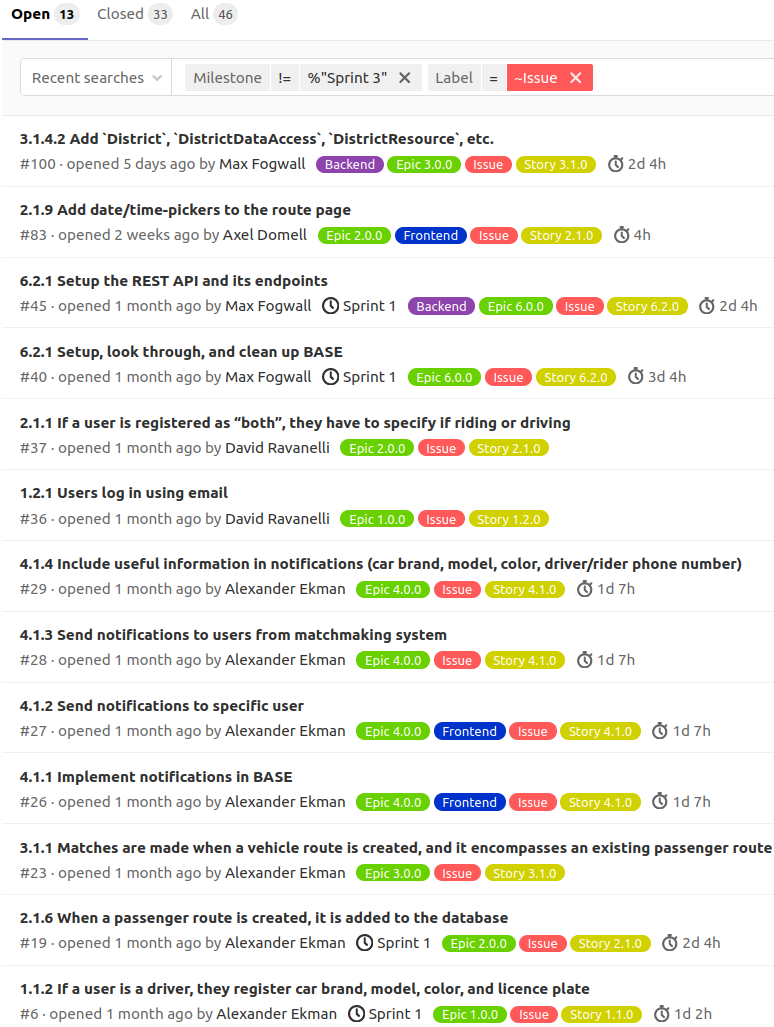
\includegraphics[scale=0.6]{pfrFigures/forgotten_issues.png}
    \caption{The list of open issues which not assigned to Sprint 3, with 1 week left of sprint 3.}
    \label{fig:forgotten_issues}
\end{figure}

\section{Summary and Future Outlook}

We had three main events that we had to deal with during the different phases. Firstly, the underestimation of story points and amount of issues. Secondly, the blocking issue and lastly, the team satisfaction. The first and second problem were dealt with by tracking the metrics and using our SDP risk analysis. The third problem was solved by tracking the metrics and having cooperation between the scrum master and the developers. These three examples show that the team overall worked in an agile fashion when faced with challenges. %This shows that the team followed the scrum structure and also how well the scrum method works.

The value of the project owners was apparent by the good planning and documentation, for example the risk analysis and structuring of the product backlog. The value of the scrum master became very clear when we could track metrics and early on catch problems. The metrics were also used in the sprint planning and in the sprint retrospective in order to improve both the way we planed and worked as a team.  The cooperation between the scrum master and the developers in the scrum methodology was also useful. This was shown when the team satisfaction problem occurred and then got resolved by the developers for sprint 3.

The scrum principles of planning and then evaluating on meetings at short intervals were also very useful. This was shown when the developers learned and improve their estimations after sprint 1. The developers also showed how useful they are in scrum when their good teamwork improved the metrics for each sprint.

Furthermore the cooperation between the product owners and the scrum master worked well, it was clear which responsibilities were joint and which were the disjoint. The PG had good communication over the course of the project which helped both feel confident in their roles. The POs expressed that they at times felt disconnected from the developers, which is a direct result of the SCRUM roles. Another result of the project's premise is that each team member only has seen the SCRUM process from one perspective. In the future, it might be beneficial to have a rotating role schedule to ensure that students get to experience more roles. 

\subsection{Dos and Don'ts}
In an effort to make the key outcomes of this project final report more accessible to future projects, we have summarised some key conclusions here:

\begin{itemize}
    \item Do split the team in smaller sub-teams
    \item Do assign a contact person for each sub-team
    \item Do not assign a sub-team responsible, in order to avoid "a neck to strangle"
    \item Do not settle for a freemium project management tool
    \item Do prioritize JIRA over a team of 13
    \item Do not use a locally hosted server of free services like GitLab, there will be limited support and features
    \item Do make time to complete the PRD and SDP before the first sprint planning. A complete use case diagram and list of requirements will be a source of many epics and user stories
    \item Do have a physical kickoff meeting. This was missing from our project, and we believe the team would have greatly benefited from this
    \item Do have time reporting working on day 1
    \item Do not let the collection of metrics outweigh the benefits of having time left over for engaging with and helping the developers
    \item Do collect team satisfaction regularly
    \item Do not exclude the product owners and scrum master from the team satisfaction survey
    \item Do contact developers based on the team satisfaction survey
    \item Do expect a large addition of open issues the first day the developers touch the project
    \item Do have weekly meetings with the client and other POs and SMs
    \item Do not have recurring meetings scheduled over lunch just because it makes scheduling easier. Use tools like "Lettuce meet" instead
    \item Do use the risk management developed in the SDP
    \item Do keep an eye on forgotten issues
    \item Do cycle students between the different roles
\end{itemize}



\end{document}